% Official VTI Research Technical Report VTI-RES-2026-03 | DOI: https://doi.org/10.5281/zenodo.24290286
\documentclass[10pt,twocolumn]{article}

\usepackage[utf8]{inputenc}
\usepackage[T1]{fontenc}
\usepackage{lmodern}
\usepackage{microtype}
\usepackage[margin=0.72in,columnsep=0.24in]{geometry}
\usepackage{amsmath,amssymb,amsfonts,mathtools}
\usepackage{booktabs,tabularx,array}
\usepackage{listings}
\usepackage{xcolor}
\usepackage{tikz}
\usetikzlibrary{arrows.meta,positioning,fit,backgrounds}
\usepackage{enumitem}
\usepackage{cite}
\usepackage[hyphens]{url}
\usepackage[colorlinks=true,linkcolor=blue!60!black,citecolor=blue!60!black,urlcolor=blue!60!black]{hyperref}

\newcolumntype{Y}{>{\raggedright\arraybackslash}X}

\lstdefinelanguage{PostgresSQL}{
  keywords={BEGIN,SELECT,INTO,STRICT,FROM,WHERE,FOR,SHARE,UPDATE,SET,AND,RETURNING,COMMIT,UNIQUE,IS,NULL},
  sensitive=false,
  morecomment=[l]{--},
  morestring=[b]'
}

\lstset{
  language=PostgresSQL,
  basicstyle=\ttfamily\scriptsize,
  keywordstyle=\bfseries\color{blue!65!black},
  commentstyle=\itshape\color{gray!70!black},
  stringstyle=\color{teal!60!black},
  frame=single,
  rulecolor=\color{black!25},
  backgroundcolor=\color{gray!4},
  columns=fullflexible,
  keepspaces=true,
  breaklines=true,
  aboveskip=0.6em,
  belowskip=0.6em,
  xleftmargin=2pt,
  xrightmargin=2pt
}

\setlength{\emergencystretch}{1.5em}

\title{\Large\bfseries Formal Blast-Radius Containment, Zero-Breakage Credential Rotation, and Epistemic Zero-Trust Isolation in Enterprise Multi-Agent Ecosystems:\\[0.25em]
\large Hypothetical Formulation, Invariant Proofs, and Technical Validation Against Peer-Reviewed Literature}

\author{%
  \textbf{Caio Gon\c{c}alves}\\
  \textit{Principal Investigator \& Chief Systems Architect, VTI Research (VTI, Brazil)}\\
  \small Technical Paper ID: \texttt{VTI-RES-2026-03} (Edition \texttt{v1.2}) \quad|\quad \url{https://projectos-system.github.io/vti-research/}
}

\date{November 2026}

\begin{document}
\nocite{R01,R02,R03,R04,R05,R06,R07,R08,R09,R10,R11,R12,R13,R14,R15,R16,R17,R18,R19,R20,R21,R22,R23,R24,R25,R26,R27,R28,R29}

\maketitle

\begin{abstract}
\noindent Transitioning from isolated Large Language Model (LLM) prototypes to continuously operating enterprise multi-agent ecosystems introduces a compound attack surface that extends far beyond prompt-level jailbreaks. When a multi-tenant cognitive hub ($\mathcal{S}_{\mathrm{Hub}}$), a daily regulatory ingestion and document-auditing portal ($\mathcal{S}_{\mathrm{Portal}}$), a local autonomous CLI orchestrator ($\mathcal{S}_{\mathrm{CLI}}$), specialized satellite microservices ($\{\mathcal{S}_{\mathrm{Sat}}^{(i)}\}_{i=1}^{k}$), and a segregated financial telemetry unit ($\mathcal{S}_{\mathrm{Obs}}$) coexist under strict zero-downtime (\emph{zero-breakage}) constraints, eight coupled vulnerability classes emerge: (i)~blast-radius amplification caused by shared upstream AI provider credentials tied to live legacy consumers; (ii)~secret persistence in version-control indices, plaintext container orchestration specifications, and destructive \emph{destroy-before-verify} deployment pipelines; (iii)~silent multimodal capability breakage (speech synthesis and transcription) following project-level model allowlisting; (iv)~prefix-regex RBAC privilege escalation, cross-channel insecure direct object references (\emph{cross-channel IDOR}), and URL-borne session token leakage in embedded iframes; (v)~confused-deputy execution, environment variable sprawl, \texttt{.git/hooks} persistence, and terminal escape injection (\texttt{OSC 52}) in autonomous CLI subprocesses; (vi)~unsigned control-plane drift, duplicate-key JSON parser differentials, post-revocation cache staleness, and orphan in-flight side effects under \emph{TOCTOU} race conditions; (vii)~recursive synthetic self-confirmation (Goodhart collapse) and retrieval-augmented generation corruption (\emph{RAG poisoning}); and (viii)~structural tension between append-only forensic audit ledgers and statutory right-to-erasure mandates over structured personal data. Employing an anonymized architectural case study design with generalized hypothetical formulation, we formalize eight falsifiable threat hypotheses ($H_1$--$H_8$), derive eight fail-closed defense-in-depth controls ($C_1$--$C_8$) with explicit formal invariants, report bounded empirical concurrency, cryptographic, and latency observations over the evaluated artifact, and critically audit both the technical validity and residual limits of each control against 29 verified peer-reviewed and normative primary references, alongside formal threats to validity and six prospective structural enhancements (\texttt{M-FUT-1}--\texttt{M-FUT-6}).

\vspace{0.5em}
\noindent\textbf{Keywords:} Zero-Trust Security; Multi-Agent LLM Systems; Blast-Radius Containment; Zero-Breakage Credential Rotation; JSON Parser Differentials (\texttt{RFC 8785}); ACID Fencing Tokens; RAG Poisoning; Cryptographic Erasure (\emph{Crypto-Shredding}).
\end{abstract}

\section{Introduction and Scientific Motivation}

Recent foundational-model systems security research reveals a decisive paradigm shift: adversarial manipulation does not need to defeat internal model weight alignment when it can exploit \emph{poorly mediated authority boundaries in the surrounding host architecture}~\cite{R22,R25,R27}. In the 2025 official release of the \emph{OWASP Top 10 for Large Language Model Applications}~\cite{R29}, systemic architectural weaknesses---including \emph{Excessive Agency} (\texttt{LLM06:2025}), \emph{Sensitive Information Disclosure} (\texttt{LLM02:2025}), \emph{Data and Model Poisoning} (\texttt{LLM04:2025}), \emph{Vector and Embedding Weaknesses} (\texttt{LLM08:2025}), and \emph{Unbounded Consumption} (\texttt{LLM10:2025})---stand alongside \emph{Prompt Injection} (\texttt{LLM01:2025}) as first-order enterprise threats.

However, existing academic literature predominantly examines each threat vector in isolation---investigating version-control secret leakage alone~\cite{R15,R20}, agent plugin execution isolation alone~\cite{R25}, or retrieval corpus poisoning alone~\cite{R26}. Within continuously operating (24/7) enterprise environments handling statutory, legal, accounting, and financial obligations, \textbf{these attack surfaces interact non-linearly}:
\begin{enumerate}[leftmargin=1.4em,itemsep=2pt,topsep=3pt]
  \item Hasty revocation of a shared upstream API credential to halt quota or data exfiltration (\texttt{LLM02}) instantaneously severs live legacy production integrations unless preceded by architectural decoupling and a telemetry-verified drain protocol (\emph{Zero-Breakage Constraint})~\cite{R20}.
  \item Enforcing strict upstream model allowlists to bound cost and third-party model risk (\texttt{LLM10}~\cite{R24,R29}) silently breaks secondary voice and accessibility pipelines whenever execution planners lack pre-flight capability verification.
  \item Prompt-level defenses (\texttt{LLM01}) become vacuous if underlying vector knowledge bases can be mutated out-of-band bypassing certification pipelines (\texttt{LLM08}~\cite{R26}), if authorization caches serve stale post-revocation responses, or if concurrent in-flight workers commit orphan database mutations after privilege revocation~\cite{R03,R13}.
\end{enumerate}

Adopting a hypothetico-deductive methodology, this paper makes three contributions: (a)~we formalize an algebraic system model $\mathcal{E}$ and an explicit adversary model capturing enterprise multi-agent ecosystems under strict zero-downtime constraints; (b)~we specify eight fail-closed defense-in-depth controls ($C_1$--$C_8$) backed by verifiable cryptographic, protocol, and ACID transactional invariants; and (c)~we subject both bounded empirical measurements and residual architectural boundaries to adversarial cross-examination against 29 primary normative and scientific sources~\cite{R01,R02,R03,R04,R05,R06,R07,R08,R09,R10,R11,R12,R13,R14,R15,R16,R17,R18,R19,R20,R21,R22,R23,R24,R25,R26,R27,R28,R29}, deriving a six-part evolutionary roadmap (\texttt{M-FUT-1}--\texttt{M-FUT-6}).

\section{Hypothetical System Model $\mathcal{E}$ and Adversary Model}

\subsection{Study Design, Strict Anonymization, and Epistemological Demarcation}

To reconcile reproducible formal security specifications with uncompromising industrial confidentiality, we adopt a \textbf{retrospective anonymized single-case architectural study with generalized hypothetical formulation}:
\begin{enumerate}[leftmargin=1.4em,itemsep=2pt,topsep=3pt]
  \item \textbf{Redacted Identifiers vs.\ Preserved Invariants:} All corporate names, commercial product identifiers, DNS domains, IP subnets, tenant identifiers, private directory paths, and literal cryptographic key prefixes were purged. We preserved with exact fidelity all \emph{topological trust boundaries}, \emph{SQL and cryptographic predicates}, \emph{protocol state machines}, and \emph{instrumented latency and concurrency measurements} obtained on the evaluated artifact.
  \item \textbf{Epistemic Proportionality ($\text{Claim Scope} \le \text{Evidence Scope}$):} Table~\ref{tab:epistemic} demarcates architectural abstraction, threat hypotheses, verified controls, and prospective designs.
  \item \textbf{Universal Fail-Closed Semantics and Telemetry Minimization:} Every control across $C_1$--$C_8$ enforces strict fail-closed semantics: primary RW database unavailability, \texttt{Ed25519} verification failure, missing pre-flight secrets, or expired epochs/tickets result in deterministic rejection (\texttt{HTTP 403/404/422/503}), never permissive bypass~\cite{R01}. Observability pipelines apply pre-persistence redaction so audit trails never become secondary leaks for secrets or raw PII.
\end{enumerate}

\begin{table*}[t]
\centering
\caption{Epistemological Demarcation and Strict Inference Boundaries ($\text{Claim Scope} \le \text{Evidence Scope}$).}
\label{tab:epistemic}
\footnotesize
\begin{tabularx}{\textwidth}{@{}l l Y Y@{}}
\toprule
\textbf{Formal Element} & \textbf{Epistemological Nature} & \textbf{Evidentiary Basis in This Study} & \textbf{Strict Inference Boundary} \\
\midrule
Topology $\mathcal{E}$ & Anonymized architectural abstraction & Structural mapping of a live enterprise production/staging ecosystem & Represents a salient class of enterprise topologies, not a market-wide prevalence survey. \\
\addlinespace[2pt]
Hypotheses $H_1$--$H_8$ & Falsifiable threat hypotheses & Attack-surface modeling + primary literature~\cite{R01,R15,R22,R25,R26,R28,R29} & Characterize structural vulnerabilities exploitable absent controls; do not claim external intrusion occurred. \\
\addlinespace[2pt]
Controls $C_1$--$C_8$ & Verified fail-closed controls & Deterministic contract suites, live SQL concurrency races, monotonic timing & Effectiveness proven under stated operational assumptions; does not imply unconditional immunity outside TCB. \\
\addlinespace[2pt]
Roadmap \texttt{M-FUT-1..6} & Prospective engineering specs & Theoretical gap analysis against frontier literature~\cite{R07,R08,R13,R16,R20,R27} & Engineering designs for subsequent maturity cycles; not yet empirically benchmarked herein. \\
\bottomrule
\end{tabularx}
\end{table*}

\subsection{Formal Topology of the Abstracted Ecosystem}

Let $\mathcal{E}$ denote a distributed enterprise ecosystem serving a finite set of tenants $\mathcal{T}$ across regulated normative domains $\mathcal{D}$, defined as:
\begin{equation}
\mathcal{E} = \left(\mathcal{S}_{\mathrm{Hub}}, \; \mathcal{S}_{\mathrm{Portal}}, \; \mathcal{S}_{\mathrm{CLI}}, \; \{\mathcal{S}_{\mathrm{Sat}}^{(i)}\}_{i=1}^{k}, \; \mathcal{S}_{\mathrm{Obs}}\right)
\end{equation}
comprising five interacting subsystems (illustrated in Figure~\ref{fig:topology}):
\begin{itemize}[leftmargin=1.3em,itemsep=2pt,topsep=3pt]
  \item $\mathcal{S}_{\mathrm{Hub}}$ (\emph{Core Cognitive \& Agentic Hub}): multi-tenant platform hosting seven specialized agent families $\mathcal{F} = \{F_1, \dots, F_7\}$ (strict normative advisory, executive copilots, commercial agents, omnichannel support, API operational assistants, SQL/BI analysts, and software engineering), backed by primary relational database $DB_{\mathrm{Hub}}$ and HNSW vector engine $DB_{\mathrm{Vec}}$.
  \item $\mathcal{S}_{\mathrm{Portal}}$ (\emph{Normative Ingestion \& Regulatory Portal}): platform ingesting dozens of official public feeds daily, auditing texts against deterministic quality criteria, running statutory calculation engines, and embedding specialized domain modules via cross-origin frames (\texttt{<iframe>}).
  \item $\mathcal{S}_{\mathrm{CLI}}$ (\emph{Autonomous CLI \& Subprocess Orchestrator}): local/hybrid orchestrator dispatching tasks across external CLI agent binaries ($a \in \{\texttt{cli}_1, \dots, \texttt{cli}_5\}$) over Git repositories and local document vaults.
  \item $\{\mathcal{S}_{\mathrm{Sat}}^{(i)}\}_{i=1}^{k}$ (\emph{Satellite Domain Microservices}): vertical domain services requiring inference and batch embeddings without architectural justification to custody upstream provider master keys from $\mathcal{P}_{\mathrm{LLM}}$.
  \item $\mathcal{S}_{\mathrm{Obs}}$ (\emph{Financial \& Administrative Observability Unit}): isolated unit dedicated solely to billing reconciliation, quota governance, and key-drain telemetry with $\mathcal{P}_{\mathrm{LLM}}$.
\end{itemize}

\begin{figure*}[t]
\centering
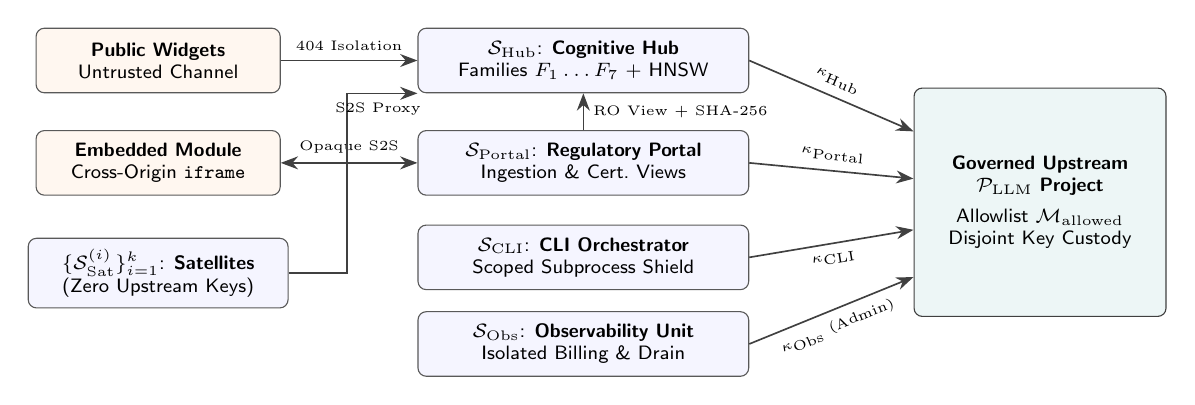
\begin{tikzpicture}[
  font=\scriptsize\sffamily,
  node distance=0.55cm and 1.1cm,
  box/.style={draw=black!65, rounded corners=3pt, fill=blue!4, minimum width=3.3cm, minimum height=0.82cm, align=center, inner sep=4pt},
  extbox/.style={draw=black!65, rounded corners=3pt, fill=orange!6, minimum width=3.1cm, minimum height=0.82cm, align=center, inner sep=4pt},
  provbox/.style={draw=black!75, rounded corners=3pt, fill=teal!7, minimum width=3.2cm, minimum height=2.9cm, align=center, inner sep=5pt},
  arr/.style={-{Stealth[length=2.2mm]}, semithick, draw=black!75},
  biarr/.style={{Stealth[length=2.2mm]}-{Stealth[length=2.2mm]}, semithick, draw=black!75}
]
  % External left
  \node[extbox] (pub) at (0, 1.55) {\textbf{Public Widgets}\\Untrusted Channel};
  \node[extbox] (emb) at (0, 0.25) {\textbf{Embedded Module}\\Cross-Origin \texttt{iframe}};
  \node[box]    (sat) at (0, -1.15) {$\{\mathcal{S}_{\mathrm{Sat}}^{(i)}\}_{i=1}^k$: \textbf{Satellites}\\(Zero Upstream Keys)};

  % Core middle
  \node[box, minimum width=4.2cm] (hub)    at (5.4, 1.55) {$\mathcal{S}_{\mathrm{Hub}}$: \textbf{Cognitive Hub}\\Families $F_1 \dots F_7$ + HNSW};
  \node[box, minimum width=4.2cm] (portal) at (5.4, 0.25) {$\mathcal{S}_{\mathrm{Portal}}$: \textbf{Regulatory Portal}\\Ingestion \& Cert.\ Views};
  \node[box, minimum width=4.2cm] (cli)    at (5.4, -0.95) {$\mathcal{S}_{\mathrm{CLI}}$: \textbf{CLI Orchestrator}\\Scoped Subprocess Shield};
  \node[box, minimum width=4.2cm] (obs)    at (5.4, -2.05) {$\mathcal{S}_{\mathrm{Obs}}$: \textbf{Observability Unit}\\Isolated Billing \& Drain};

  % Provider right
  \node[provbox] (pllm) at (11.2, -0.25) {\textbf{Governed Upstream}\\$\mathcal{P}_{\mathrm{LLM}}$ \textbf{Project}\\[0.4em]Allowlist $\mathcal{M}_{\mathrm{allowed}}$\\Disjoint Key Custody};

  % Edges
  \draw[arr]   (pub.east) -- node[above, font=\tiny]{404 Isolation} (hub.west);
  \draw[biarr] (emb.east) -- node[above, font=\tiny]{Opaque S2S} (portal.west);
  \draw[arr]   (sat.east) -- (2.4,-1.15) |- node[pos=0.72, below, font=\tiny]{S2S Proxy} (hub.south west);
  \draw[arr]   (portal.north) -- node[right, font=\tiny]{RO View + SHA-256} (hub.south);

  \draw[arr] (hub.east)    -- node[above, sloped, font=\tiny]{$\kappa_{\mathrm{Hub}}$} ([yshift=0.9cm]pllm.west);
  \draw[arr] (portal.east) -- node[above, sloped, font=\tiny]{$\kappa_{\mathrm{Portal}}$} ([yshift=0.3cm]pllm.west);
  \draw[arr] (cli.east)    -- node[below, sloped, font=\tiny]{$\kappa_{\mathrm{CLI}}$} ([yshift=-0.35cm]pllm.west);
  \draw[arr] (obs.east)    -- node[below, sloped, font=\tiny]{$\kappa_{\mathrm{Obs}}$ (Admin)} ([yshift=-0.95cm]pllm.west);
\end{tikzpicture}
\caption{Formal Zero-Trust Topology of Abstracted Enterprise Multi-Agent Ecosystem $\mathcal{E}$.}
\label{fig:topology}
\end{figure*}

\subsection{Adversary Model and Weighted Blast Radius}

\textbf{Adversary Capabilities ($\mathcal{A}$):} We consider a composite adversary spanning four realistic vectors: (a)~\emph{External Web/Network Attacker}, interacting arbitrarily with public widgets, inspecting browser history/\texttt{Referer} headers, spoofing unverified HTTP headers (\texttt{Origin}, \texttt{x-user-login}), probing session UUIDs, and launching sub-millisecond concurrent HTTP races; (b)~\emph{Indirect Epistemic Adversary}, injecting malicious instructions into external regulatory documents, web pages, or repository artifacts read by $\mathcal{S}_{\mathrm{Hub}}$ or $\mathcal{S}_{\mathrm{CLI}}$ (targeting indirect prompt injection, \texttt{.git/hooks} persistence, \texttt{OSC 52} clipboard hijacking, or \emph{PoisonedRAG})~\cite{R22,R26}; (c)~\emph{Localized Peripheral Compromise}, disclosing configuration in a build artifact, legacy \texttt{.env} file, or satellite container $\mathcal{S}_{\mathrm{Sat}}^{(i)}$; and (d)~\emph{Out-of-Band Mutation or Concurrency Race}, comprising permission revocations racing against in-flight agent executions or direct manual SQL edits on base tables. Our Trusted Computing Base (TCB) assumes standard cryptographic primitives (\texttt{SHA-256}, \texttt{Ed25519}, \texttt{AES-256-GCM}, OS CSPRNG), primary PostgreSQL ACID integrity, and an uncompromised host supervisor kernel.

\textbf{Weighted Blast-Radius Metric:} Let $\mathcal{K}$ be the set of active credentials and $\mathcal{W} = \{w_1, \dots, w_m\}$ be production workloads with criticality $\omega_r > 0$, maximum bounded financial exposure $C_{\max}(w_r)$, and risk scalar $\lambda > 0$. With $\mathrm{Uses}(w_r, \kappa) \in \{0, 1\}$ indicating whether compromise or emergency revocation of $\kappa \in \mathcal{K}$ directly impacts $w_r$, the \textbf{Operational-Financial Blast Radius} is:
\begin{equation}
\mathrm{BR}(\kappa) = \sum_{r=1}^{m} \mathrm{Uses}(w_r, \kappa) \cdot \left(\omega_r + \lambda C_{\max}(w_r)\right)
\end{equation}
Under the \emph{Monolithic Credential Null Hypothesis} ($\kappa_{\mathrm{shared}}$ shared across all subsystems plus an uninterrupted legacy consumer $w_{\mathrm{crit}}$), $\mathrm{BR}(\kappa_{\mathrm{shared}}) = \sum_{r=1}^{m} (\omega_r + \lambda C_{\max}(w_r))$ reaches the worst-case theoretical maximum: any peripheral leak forces either tolerating global quota/data drain or revoking $\kappa_{\mathrm{shared}}$ and breaking $w_{\mathrm{crit}}$. Table~\ref{tab:hypotheses} summarizes the eight threat hypotheses $H_1$--$H_8$.

\begin{table*}[t]
\centering
\caption{Summary of the Eight Falsifiable Threat Hypotheses ($H_1$--$H_8$) Over Ecosystem $\mathcal{E}$.}
\label{tab:hypotheses}
\footnotesize
\begin{tabularx}{\textwidth}{@{}c l Y@{}}
\toprule
\textbf{ID} & \textbf{Vulnerability Class (\texttt{CWE} / \texttt{OWASP LLM 2025})} & \textbf{Formal Risk Statement Over Ecosystem $\mathcal{E}$} \\
\midrule
$H_1$ & Shared Upstream Key \& Rotation Deadlock (\texttt{CWE-798}, \texttt{LLM02/10}) & Sharing $\kappa_{\mathrm{shared}}$ couples all subsystem blast radii and blocks immediate revocation when critical consumer $w_{\mathrm{crit}}$ shares the secret. \\
\addlinespace[2pt]
$H_2$ & VCS Persistence, Plaintext Specs \& \emph{Destroy-Before-Verify} (\texttt{CWE-312/522}) & Tracked \texttt{.env} files, plaintext container specs, and tearing down active stacks prior to secret checks cause leakage or deploy outages. \\
\addlinespace[2pt]
$H_3$ & Post-Allowlist Multimodal Breakage (\texttt{LLM10}, Model Governance) & Restricting upstream models to $\mathcal{M}_{\mathrm{allowed}}$ silently breaks speech (\texttt{TTS/STT}) calls without pre-flight probing and governed fallback. \\
\addlinespace[2pt]
$H_4$ & Prefix RBAC, \emph{Cross-Channel IDOR} \& URL Tokens (\texttt{CWE-285/639/598}) & Prefix regexes (\texttt{/\^{}prefix\_/i}), unmediated public session resumption, and query-string tickets enable privilege escalation and \texttt{Referer} leaks. \\
\addlinespace[2pt]
$H_5$ & \emph{Confused Deputy} \& CLI Persistence (\texttt{CWE-441}, \texttt{CWE-88}, \texttt{LLM06}) & Inheriting full \texttt{process.env} exposes cross-service secrets and enables persistence via \texttt{.git/hooks/*} or ANSI \texttt{OSC 52} clipboard hijacking. \\
\addlinespace[2pt]
$H_6$ & \emph{Parser Differentials}, Stale Cache \& \emph{TOCTOU} (\texttt{CWE-436}, \texttt{CWE-367}) & Duplicate JSON keys cause verifier-executor divergence; epoch-blind caches serve revoked data; concurrent revocations yield orphan writes. \\
\addlinespace[2pt]
$H_7$ & Recursive Goodhart Collapse \& \emph{PoisonedRAG} (\texttt{LLM04}, \texttt{LLM08}) & Re-ingesting synthetic outputs as independent corroboration or direct SQL base-table edits corrupts the retrieved normative corpus. \\
\addlinespace[2pt]
$H_8$ & Structured PII vs.\ Audit Immutability (\texttt{LLM02}, \texttt{GDPR/LGPD}) & Naive digit regexes corrupt valid contract IDs or leak PII into embeddings, while append-only ledgers conflict with erasure mandates. \\
\bottomrule
\end{tabularx}
\end{table*}

\section{Formulation of Threat Hypotheses ($H_1$--$H_8$) and Fail-Closed Controls ($C_1$--$C_8$)}

\subsection{Control $C_1$ (for $H_1$): Domain Partitioning, Zero-Key S2S Proxy, and Dual-Key Grace Window}

\textbf{1. Disjoint Credential Partitioning:} Within the governed upstream project $\mathcal{P}_{\mathrm{LLM}}$, keys are partitioned into strictly disjoint sets:
\begin{equation}
\begin{aligned}
\mathcal{K}_{\mathrm{inference}} &= \{\kappa_{\mathrm{Hub}}, \; \kappa_{\mathrm{Portal}}, \; \kappa_{\mathrm{CLI}}\}, \quad
\mathcal{K}_{\mathrm{admin}} = \{\kappa_{\mathrm{Obs}}\},\\
\kappa_a &\neq \kappa_b \quad (\forall a \neq b)
\end{aligned}
\end{equation}
where $\kappa_{\mathrm{Obs}}$ resides solely in $\mathcal{S}_{\mathrm{Obs}}$ with zero inference scope on application nodes.

\textbf{2. Zero Upstream Keys in Satellites ($\mathrm{BR}_{\mathrm{upstream}}(\mathcal{S}_{\mathrm{Sat}}^{(i)}) = 0$):} Satellites $\{\mathcal{S}_{\mathrm{Sat}}^{(i)}\}_{i=1}^{k}$ hold no $\mathcal{P}_{\mathrm{LLM}}$ keys; inference and batch embeddings ($B \le 64$) traverse an authenticated S2S proxy on $\mathcal{S}_{\mathrm{Hub}}$ where model selection remains server-\texttt{LOCKED} (\texttt{ON CONFLICT DO NOTHING} over centrally governed parameters).

\textbf{3. Dual-Key Grace Window:} For a live legacy consumer $w_{\mathrm{crit}}$ coupled to $\kappa_{\mathrm{legacy}}$: Phase~1 atomically migrates $\mathcal{S}_{\mathrm{Hub}}$, $\mathcal{S}_{\mathrm{Portal}}$, and $\mathcal{S}_{\mathrm{CLI}}$ to disjoint keys, reducing $\mathrm{BR}(\kappa_{\mathrm{legacy}})$ to $\omega_{\mathrm{crit}} + \lambda C_{\max}(w_{\mathrm{crit}})$; Phase~2 holds $\kappa_{\mathrm{legacy}}$ in state \texttt{RETIRING} under $\mathcal{S}_{\mathrm{Obs}}$ telemetry until $\lambda_{\mathrm{req}}(\kappa_{\mathrm{legacy}}, \Delta t) = 0$ for $\Delta t \ge \Delta_{\mathrm{drain}}$ post-connector update, resolving industry rotation paralysis~\cite{R01,R16,R20}.

\subsection{Control $C_2$ (for $H_2$): Ephemeral \texttt{tmpfs} Secrets and Verify-Before-Destroy CI Gate}

Sensitive credentials migrate from plaintext container environment specs into immutable RAM-backed \texttt{tmpfs} mounts (\texttt{/run/secrets/*})~\cite{R18}. To prevent stack destruction when secrets are missing, CI/CD enforces the blocking pre-flight invariant:
\begin{equation}
\mathrm{PreFlightOK}(S_{\mathrm{req}}) \iff \forall s \in S_{\mathrm{req}}, \;\; s \in \mathrm{ClusterSecretStore}()
\end{equation}
aborting prior to any mutating orchestrator command if $\neg \mathrm{PreFlightOK}(S_{\mathrm{req}})$. Entrypoint hydration strips \texttt{\textbackslash r\textbackslash n} and enforces $\mathrm{len}(\mathrm{trim}(\mathrm{val})) > 0$, while legacy build stages truncate \texttt{.env} placeholders to zero bytes (\texttt{: > .env}) prior to packaging~\cite{R15,R21}.

\subsection{Control $C_3$ (for $H_3$): Pre-Deployment Allowlist Probing and Capability Registry}

Before release under upstream allowlist $\mathcal{M}_{\mathrm{allowed}}$ ($|\mathcal{M}_{\mathrm{allowed}}| = 49$), pre-flight probes (\texttt{GET /v1/models}) verify $\mathcal{M}_{\mathrm{configured}} \subseteq \mathcal{M}_{\mathrm{allowed}}$. At runtime, \texttt{ModelCapabilityRegistry} bifurcates policy~\cite{R24,R29}: (i)~high-stakes normative/analytical families ($F_1, F_6, F_7$) fail closed (\texttt{HTTP 422 CapabilityMismatch}) rather than silently downgrading reasoning effort, natively selecting structured transport (\texttt{/v1/responses} with \texttt{store: false}) whenever \texttt{effort != 'none'}; (ii)~voice channels (\texttt{TTS/STT}) execute audited fallback strictly within $\mathcal{M}_{\mathrm{audio}} \cap \mathcal{M}_{\mathrm{allowed}}$.

\subsection{Control $C_4$ (for $H_4$): Enumerated RBAC, Cross-Channel Isolation, and Opaque Handshake}

\textbf{1. Closed-Set RBAC:} Replacing prefix regexes (\texttt{/\^{}prefix\_/i}), administrative privilege is evaluated strictly over finite sets using verified JWT claims alone:
\begin{equation}
\mathrm{isAdmin}(r) \iff \mathrm{lower}(r) \in \mathcal{R}_{\mathrm{admin\_allow}} \setminus \mathcal{R}_{\mathrm{client\_explicit\_deny}}
\end{equation}

\textbf{2. Cross-Channel Indistinguishability:} Public widget resumption enforces immutable creation-channel mediation:
\begin{equation}
\begin{aligned}
\mathrm{CanResumePublic}(c, \mathrm{hdr}_{\mathrm{origin}}) \iff{} & \mathrm{origin}(c) = \texttt{PUBLIC\_WIDGET}\\
&\land\; \mathrm{agentType}(c) \neq \texttt{API\_ASSISTANT}\\
&\land\; \mathrm{hdr}_{\mathrm{origin}} \in \mathrm{AllowedOrigins}(c)
\end{aligned}
\end{equation}
returning uniform \texttt{HTTP 404 Not Found} on any violation~\cite{R01,R05}.

\textbf{3. Reverse Opaque PostMessage Handshake (\texttt{RFC 9700}):} Cross-origin \texttt{<iframe>} modules load neutral \texttt{/embed/bootstrap}, generate a CSPRNG \texttt{handshakeNonce}, receive an in-memory opaque ticket $t_{\mathrm{opaque}}$ (\texttt{TTL = 60 s}) via \texttt{postMessage}, and redeem it via constant-time authenticated S2S backchannel (\texttt{timingSafeEqual}) using a single atomic SQL statement~\cite{R28}:
\begin{lstlisting}
UPDATE embedded_opaque_tickets
   SET consumed_at = statement_timestamp()
 WHERE token_hash = $1
   AND consumed_at IS NULL
   AND expires_at > statement_timestamp()
   AND handshake_nonce = $2
   AND embed_origin = $3
RETURNING ticket_id, user_id, tool_scope;
\end{lstlisting}
where \texttt{statement\_timestamp()} prevents long-transaction skew, \texttt{rowCount === 1} is verified pre-commit (\texttt{ROLLBACK} otherwise), and narrow-scoped tokens (\texttt{scope = 'embedded\_module'}) are emitted strictly post-\texttt{COMMIT}.

\subsection{Control $C_5$ (for $H_5$): Execution Shield for Autonomous CLI Agents}

Subprocess binaries $a \in \{\texttt{cli}_1, \dots, \texttt{cli}_5\}$ are confined against indirect prompt injection~\cite{R22,R25} via:
\begin{equation}
\mathrm{Env}(a) = \left(\mathrm{Env}_{\mathrm{host}} \upharpoonright \mathcal{A}_{\mathrm{sys\_safe}}\right) \cup \mathrm{Creds}_{\mathrm{authorized}}(a) \setminus \mathcal{B}_{\mathrm{hard\_blocked}}
\end{equation}
stripping host UI tokens, cloud/DB secrets, and hijack vectors (\texttt{NODE\_OPTIONS}, \texttt{GIT\_SSH\_COMMAND}, \texttt{GIT\_ASKPASS}, \texttt{GIT\_CONFIG\_*}). Pre- and post-turn \texttt{SHA-256} snapshots atomically restore unauthorized mutations to \texttt{.git/config} and \texttt{.git/hooks/*} prior to host \texttt{git} calls (invoked with \texttt{-c core.hooksPath= -c core.fsmonitor=false -c protocol.file.allow=never}). Terminal streams strip \texttt{OSC 52} and \texttt{DCS/APC/PM} escapes, while audit records $R_n$ use injective binary length framing~\cite{R04}:
\begin{multline}
H_n = \mathrm{SHA256}\Bigl(\texttt{audit:ledger:v1\textbackslash 0} \parallel H_{n-1}^{[32\text{B}]} \\
\parallel \mathrm{uint64\_be}\!\left(\lvert \mathrm{JCS}(R_n) \rvert_{\mathrm{bytes}}\right) \parallel \mathrm{JCS}(R_n)\Bigr)
\end{multline}
anchoring $(n, H_n)$ inside a supervisor database inaccessible to the CLI subprocess.

\subsection{Control $C_6$ (for $H_6$): Lexical JSON Guard, Epoch Cache, and ACID Fencing}

\textbf{1. Anti-Parser-Differential Signing:} Raw JSON text is lexically scanned prior to AST construction, aborting (\texttt{ERR\_DUPLICATE\_JSON\_KEY}) on duplicate keys~\cite{R12,R19} and enforcing canonical 64-bit decimal integers ($\le 2^{64}-1$) before \texttt{RFC 8785} JCS canonicalization~\cite{R17} and \texttt{Ed25519} signing~\cite{R11} over $m = (\mathrm{issuer}, \mathrm{audience}, \mathrm{schema\_version}, \mathrm{epoch}, \mathrm{iat}, \mathrm{exp}, \mathrm{key\_id}, \mathrm{payload\_hash})$.

\textbf{2. Epoch-Scoped Cache ($O(1)$ Invalidation):}
\begin{multline}
K_{\mathrm{cache}} = \mathrm{SHA256}\Bigl(\mathrm{JCS}\bigl(\mathrm{tenant}, \mathrm{callerRole}, \mathrm{scope},\\
\mathrm{epoch}_{\mathrm{manifest}}, \mathrm{epoch}_{\mathrm{authz}}, \mathrm{epoch}_{\mathrm{revoc}}, \mathrm{queryNorm}\bigr)\Bigr)
\end{multline}

\textbf{3. Four-Checkpoint Revocation and Explicit \texttt{CP-2B} Serialization:} To eliminate orphan writes and \texttt{EvalPlanQual} ambiguity under PostgreSQL \texttt{READ COMMITTED}~\cite{R03,R13}, all mutating transactions obey global lock order \texttt{control\_plane\_state} $\to$ \texttt{resource\_target} with monotonic epoch guard $e_{\mathrm{req}}$ (\texttt{\$2}):
\begin{lstlisting}
BEGIN;
SELECT current_revocation_epoch INTO STRICT v_curr_epoch
  FROM control_plane_state
 WHERE singleton_id = 1
   FOR SHARE;

UPDATE resource_target
   SET state = $1,
       applied_epoch = $2
 WHERE id = $3
   AND $2 = v_curr_epoch
   AND applied_epoch < $2
RETURNING id, applied_epoch;
COMMIT;
\end{lstlisting}
Concurrent administrative revocations serialize directly on \texttt{singleton\_id = 1}; stale workers observe \texttt{rowCount = 0} and \texttt{ROLLBACK} with zero local orphan commits.

\subsection{Control $C_7$ (for $H_7$): Acyclic Provenance, Read-Time Hash View, and Dual Sign-Off}

To prevent synthetic collapse~\cite{R23} and \emph{PoisonedRAG}~\cite{R26}, candidate artifacts carry HMAC-JCS provenance graphs validated in $O(|V| + |E|)$ via Tarjan's SCC algorithm~\cite{R02}, requiring primary official source lineage (\texttt{coleta\_oficial\_id IS NOT NULL}). $\mathcal{S}_{\mathrm{Hub}}$ queries $\mathcal{S}_{\mathrm{Portal}}$ solely via a read-only role (\texttt{default\_transaction\_read\_only = on}) over contractual views enforcing:
\begin{equation}
\begin{aligned}
\mathrm{Eligible}(d) \iff{} & (\mathrm{score}_{\mathrm{audit}}(d) = 100) \land \mathrm{hasOfficialSource}(d)\\
&\land \neg\mathrm{hasOpenDiscrepancy}(d)\\
&\land \bigl(\mathrm{SHA256}(\mathrm{canonical}(d)) = d.\mathrm{certified\_hash}\bigr)
\end{aligned}
\end{equation}
expelling any out-of-band base-table edit in \texttt{0 ms}. External oracle rules require physical two-person sign-off (\texttt{CHECK (reviewer\_a\_id <> reviewer\_b\_id)} on \texttt{version\_sha256}) under queue utilization $\varrho_q \le 0.80$~\cite{R08}.

\subsection{Control $C_8$ (for $H_8$): Algebraic Modulo-11 Filter and Per-Subject Crypto-Erasure}

Pre-indexing sanitization validates 11/14-digit check digits in \texttt{Modulo-11} arithmetic (rejecting repdigits $\texttt{d}^{11}$ while preserving benign contract/protocol numbers), plus 44-digit fiscal keys, emails, and phones prior to embedding. Reversible subject records use \texttt{AES-256-GCM} (128-bit tag) with per-subject $\mathrm{DEK}_u \in \{0,1\}^{256}$ wrapped by master $\mathrm{KEK}$~\cite{R06,R09}: (a)~96-bit CSPRNG nonces enforce rotation at $q_{\max} \le 2^{32}$ ($q(q-1)/2^{97} \le 2^{-33}$ per \texttt{NIST SP 800-38D}~\cite{R09}); (b)~canonical $\mathrm{AAD} = \mathrm{JCS}(\mathrm{schema\_v}, \mathrm{purpose}, \mathrm{key\_id}, \mathrm{tenant\_id}, \mathrm{subject\_id}, \mathrm{record\_id})$ is reconstructed from trusted context; and (c)~upon statutory erasure, destroying all recoverable copies of $\mathrm{DEK}_u$ across vaults, caches, swap, and backups renders historical ciphertexts computationally unrecoverable~\cite{R10,R14} while recording an append-only tombstone (\texttt{SQLSTATE 55000}).

\section{Bounded Empirical Observations}

We executed deterministic contract suites, sub-millisecond S2S ticket redemption races, unauthorized \texttt{.git/hooks} and \texttt{OSC 52} injections, 20-way concurrent CAS manifest bursts, live revocations racing against \texttt{CP-2B}, 1-byte out-of-band SQL edits, and P95 HNSW searches across 374,252 vectors under concurrent ingestion (Table~\ref{tab:empirical}). Amortizing asymmetric \texttt{Ed25519} verification at startup (\texttt{250.48 ms} for 11 manifests) keeps per-turn local CPU security overhead below \texttt{0.70 ms} and vector retrieval impact at \texttt{+2.852 ms} (\texttt{0.19\%}).

\begin{table*}[t]
\centering
\caption{Summary of Bounded Empirical Concurrency, Cryptographic, and Latency Observations.}
\label{tab:empirical}
\footnotesize
\begin{tabularx}{\textwidth}{@{}l Y c l@{}}
\toprule
\textbf{Evaluated Control} & \textbf{Instrumented Experimental Metric} & \textbf{Observed Result} & \textbf{Verified Operational Invariant} \\
\midrule
$C_1$ --- Satellite Blast Radius & Upstream provider keys present in $\{\mathcal{S}_{\mathrm{Sat}}^{(i)}\}$ & \textbf{0 keys} (100\% S2S) & $\mathrm{BR}_{\mathrm{upstream}}(\mathcal{S}_{\mathrm{Sat}}^{(i)}) = 0$ \\
$C_1$ --- Zero-Breakage Rotation & Errors/drops in live consumers during key split & \textbf{0 interruptions} & Continuous \texttt{HTTP 200} cutover \\
$C_2$ --- Pre-Flight Gate \& \texttt{tmpfs} & Plaintext secret env vars in orchestrator spec & \textbf{0 exposed} (100\% \texttt{/run/secrets}) & Volatile RAM + pre-destroy gate \\
$C_4$ --- Channel \& \texttt{iframe} Isolation & Public internal-session probes / tokens in URLs & \textbf{100\% 404 / 0 URL tokens} & \texttt{RFC 9700} compliance \\
$C_5$ --- CLI Execution Shield & Cross-agent env leaks / surviving tampered hooks & \textbf{0 leaks / 100\% restored} & Per-turn subprocess confinement \\
$C_6$ --- Boot \texttt{Ed25519 + JCS} & Startup verification across 11 signed manifests & \textbf{250.48 ms} (0 ms/turn) & Fail-closed boot amortization \\
$C_6$ --- Live Governance Sync & Block/model propagation on primary RW store & \textbf{374 ms} ($\le 2,000\text{ ms}$) & Sub-second primary convergence \\
$C_6$ --- CAS \& Idempotency & 20 concurrent writes / 5 parallel human clicks & \textbf{20/20 ordered / 5$\to$1 write} & Zero lost updates \\
$C_6$ --- \texttt{CP-2B} Fencing \& Rollback & Orphan commits under revocation / canary rollback & \textbf{0 orphans / 0.195 ms} & Strict ACID serialization \\
$C_7$ --- Direct SQL Tampering & Manual 1-char edit on base table outside pipeline & \textbf{0 ms expulsion} & Query-time \texttt{SHA-256} view \\
$C_7$ --- Vector Ingest Isolation & P95 overhead on 374,252 HNSW vectors under ingest & \textbf{+2.852 ms} (\textbf{0.19\%}) & Serving isolation ($\le 3\%$) \\
$C_8$ --- Modulo-11 \& Shredding & Structured PII residue / post-erasure \texttt{DEK} reads & \textbf{0 residues / 100\% opaque} & Algebraic filter \& crypto-erasure \\
\bottomrule
\end{tabularx}
\end{table*}

\section{Critical Validation Against Primary Literature and Roadmap (\texttt{M-FUT-1}--\texttt{M-FUT-6})}

\subsection{Formally Closed Properties vs.\ Residual Frontiers}

Controls $C_1$--$C_8$ formally close: (1)~duplicate-key JSON validate-vs-execute differentials~\cite{R11,R12,R17,R19} ($C_6$); (2)~browser URL/history/\texttt{Referer} token exposure~\cite{R28} ($C_4$); and (3)~local split-brain mutations inside the primary PostgreSQL database~\cite{R13} ($C_6$/\texttt{CP-2B}). Table~\ref{tab:mfut} specifies six prospective enhancements (\texttt{M-FUT-1}--\texttt{M-FUT-6}) addressing residual boundaries identified in primary literature, and Table~\ref{tab:traceability} establishes full scientific traceability across \texttt{[R01]}--\texttt{[R29]}.

\begin{table*}[t]
\centering
\caption{Six Residual Frontiers and Prospective Architectural Enhancements (\texttt{M-FUT-1} to \texttt{M-FUT-6}).}
\label{tab:mfut}
\footnotesize
\begin{tabularx}{\textwidth}{@{}c Y l Y@{}}
\toprule
\textbf{Code} & \textbf{Residual Boundary Identified in Literature} & \textbf{Primary Grounding} & \textbf{Specified Next-Cycle Enhancement} \\
\midrule
\texttt{M-FUT-1} & Static \texttt{/run/secrets} require rolling restarts to rotate; shared internal S2S secrets risk replay under satellite memory compromise. & NIST SP 800-207~\cite{R16}; RFC 9700~\cite{R28} & Internal \textbf{mTLS} (short-lived X.509 SPIFFE/SPIRE) or \textbf{DPoP} sender-constrained S2S tokens + dual-window hot rotation. \\
\addlinespace[2pt]
\texttt{M-FUT-2} & Untracking \texttt{.env} at \texttt{HEAD} and zero-byte builder truncation do not erase historical commits in \texttt{.git/objects}. & Meli et al.~\cite{R15}; Basak et al.~\cite{R20} & Audited \texttt{git filter-repo} history sanitization + 100\% historical key rotation + \textbf{BuildKit} \texttt{--mount=type=secret}. \\
\addlinespace[2pt]
\texttt{M-FUT-3} & Tool allowlists cannot stop indirect prompt injections from smuggling sensitive data inside \emph{arguments} of permitted outbound tools. & \emph{CaMeL}~\cite{R27}; Greshake et al.~\cite{R22} & Argument-level \textbf{provenance taint capabilities} blocking untrusted evidence from populating outbound recipients/URLs without out-of-LLM approval. \\
\addlinespace[2pt]
\texttt{M-FUT-4} & \texttt{Modulo-11} strips structured IDs, but rare narrative attribute combinations risk violating $k$-anonymity or vector inversion. & Sweeney~\cite{R07}; OWASP \texttt{LLM08}~\cite{R29} & Local \textbf{NER + rare monetary/geographic generalization} pre-embedding with strict per-tenant vector partitioning. \\
\addlinespace[2pt]
\texttt{M-FUT-5} & \texttt{CP-2B} rolls back PostgreSQL mutations, but external non-transactional HTTP APIs cannot join SQL \texttt{ROLLBACK} post-transmission. & Kleppmann~\cite{R13}; Lamport~\cite{R03} & \textbf{Transactional Outbox} with short cancellable hold-buffers (\texttt{2--5 s}) and idempotent compensation sagas. \\
\addlinespace[2pt]
\texttt{M-FUT-6} & Bounding queue load ($\varrho_q \le 0.80$) prevents overload, but experienced reviewers face longitudinal vigilance decrement. & Parasuraman \& Manzey~\cite{R08} & Continuous blind \textbf{seeded canary audit items} (\texttt{2\%--3\%} volume) inside dual-human sign-off queues. \\
\bottomrule
\end{tabularx}
\end{table*}

\begin{table*}[t]
\centering
\caption{Scientific Traceability Matrix Mapping Hypotheses and Controls to Verified Sources (\texttt{[R01]}--\texttt{[R29]}).}
\label{tab:traceability}
\footnotesize
\begin{tabularx}{\textwidth}{@{}l l Y@{}}
\toprule
\textbf{Hypothesis \& Control} & \textbf{Linked Primary Sources} & \textbf{Exact Scope Substantiated by Primary Literature} \\
\midrule
$H_1, C_1$ --- Key split, S2S \& Drain & \cite{R01,R16,R20} & Least privilege, centralized Policy Enforcement Point, zero-breakage rotation. \\
$H_2, C_2$ --- \texttt{tmpfs} \& Pre-Flight Gate & \cite{R15,R18,R21} & Longitudinal Git secret persistence, static scanner limits, volatile secret custody. \\
$H_3, C_3$ --- Allowlist \& Capability Reg. & \cite{R24,R29} & Pre-deployment third-party AI model governance and availability protection. \\
$H_4, C_4$ --- Enumerated RBAC \& \texttt{iframe} & \cite{R01,R05,R28} & Complete mediation, cross-channel Confused Deputy prevention, URL-free OAuth BCP. \\
$H_5, C_5$ --- CLI Shield \& Hash Framing & \cite{R04,R22,R25,R27} & Subprocess execution isolation, injective length-prefixed hashing, taint boundary. \\
$H_6, C_6$ --- JCS, Ed25519 \& \texttt{CP-2B} & \cite{R03,R11,R12,R13,R17,R19} & JSON duplicate-key differentials, canonical EdDSA signing, ACID fencing tokens. \\
$H_7, C_7$ --- Tarjan DAG \& Hash View & \cite{R02,R08,R23,R26} & Linear cycle detection, anti-collapse lineage, \emph{PoisonedRAG} defense, dual review. \\
$H_8, C_8$ --- Modulo-11 \& AEAD Erasure & \cite{R06,R07,R09,R10,R14,R29} & Bounded-nonce GCM with canonical AAD, conditional crypto-erasure, $k$-anonymity. \\
\bottomrule
\end{tabularx}
\end{table*}

\section{Threats to Validity}

\textbf{Construct Validity:} Compliance with $C_1$--$C_8$ represents continuous contextual mediation and blast-radius containment~\cite{R16}, not unconditional immunity. Hash chains ($C_5$) provide tamper-evidence conditioned on supervisor anchor isolation, and cryptographic erasure ($C_8$) holds strictly under effective destruction of all recoverable copies of $\mathrm{DEK}_u$ across vaults, caches, swap, and backups~\cite{R10}.

\textbf{Internal Validity:} Because defense-in-depth layers overlap along execution paths (e.g., scoped env + \texttt{SHA-256} \texttt{.git} restoration + \texttt{OSC 52} filtering in $C_5$), zero observed violations reflect joint suite efficacy under intact host kernels and software supply chains.

\textbf{External Validity:} Empirical latencies reflect a generalized regulatory enterprise topology backed by primary PostgreSQL ACID storage and a 374,252-vector HNSW index; non-transactional datastores or self-hosted models require threshold recalibration.

\textbf{Conclusion Validity and Reproducibility:} While proprietary production code remains anonymized, independent reproducibility is ensured via closed-form predicates, atomic SQL transactions, canonical cryptographic specs~\cite{R09,R11,R17}, and full traceability across~\cite{R01,R02,R03,R04,R05,R06,R07,R08,R09,R10,R11,R12,R13,R14,R15,R16,R17,R18,R19,R20,R21,R22,R23,R24,R25,R26,R27,R28,R29}.

\section{Conclusion}

Securing 24/7 enterprise multi-agent ecosystems requires unifying distributed systems isolation, canonical cryptography, and epistemic governance. Integrating disjoint credential partitioning with zero-breakage draining ($C_1, C_2$), pre-flight multimodal governance ($C_3$), enumerated RBAC and URL-free opaque handshakes ($C_4$), CLI subprocess confinement ($C_5$), lexically unambiguous signed manifests with epoch caching and explicit ACID fencing ($C_6$), acyclic read-verified RAG provenance ($C_7$), and algebraic \texttt{Modulo-11} de-identification with per-subject cryptographic erasure ($C_8$) yields an auditable Zero-Trust architecture adding under \texttt{1 ms} of local CPU latency and \texttt{0.2\%} vector retrieval overhead while charting six rigorous engineering milestones (\texttt{M-FUT-1}--\texttt{M-FUT-6}).

\section*{Transparent Disclosure of Symbiotic Human-AI Engineering, Deterministic Verification, and Adapted CRediT Mapping (ACM / IEEE / COPE Compliance)}

In strict compliance with \textbf{COPE}, \textbf{ACM} (\emph{Policy on Authorship}, 2023), and \textbf{IEEE} (\emph{PSPB Operations Manual}) policies, automated systems and generative models cannot hold authorship or bear ethical/legal accountability. \textbf{Caio Gon\c{c}alves} stands as the \textbf{sole formal author}, assuming undivided responsibility for all formulations, architectural specifications, empirical claims, and conclusions. Under strict \emph{Human-in-the-Loop} governance: (1)~\textbf{Caio Gon\c{c}alves} (\emph{Principal Investigator \& Chief Systems Architect, VTI Research}) led \emph{Conceptualization, Methodology, Security Architecture, Supervision, Validation, Project Administration, and Final Writing}; (2)~two rounds of non-authorial adversarial stress-testing were conducted using \emph{independent cross-family frontier and compact reasoning models} to probe formal edge cases (\texttt{statement\_timestamp()} pre-commit checks in $C_4$, \texttt{uint64\_be} injective framing in $C_5$, ordered \texttt{FOR SHARE} serialization in \texttt{CP-2B} $C_6$, and CSPRNG nonce bounds in $C_8$), with every refinement audited and deterministically verified by the human author; and (3)~all 29 references, SQL predicates, and strict anonymization invariants were deterministically verified prior to release.

\bibliographystyle{unsrt}
\bibliography{references}

\end{document}
